% !TEX root = paper.tex
% !TEX encoding = UTF-8 Unicode
% -*- coding: UTF-8; -*-
% vim: set fenc=utf-8
% !TEX spellcheck = en-US
%=================================================================
\section{Results}
\label{sec:results}
%=================================================================
%=================================================================
\subsection{Inferring where to look}
%=================================================================
After training the network, we evaluated simulations of the final accuracy at the landing of the predicted saccade (see Figure~\ref{fig:results}). For each different visual display (a different digit at a different position), a retinocentric visual input is processed (figure \ref{fig:results}-A), providing a predicted accuracy map (figure \ref{fig:results}-B) that can be compared to the actual future accuracy. Then a saccade is carried out based on the most probable position as computed from the predicted accuracy map (figure \ref{fig:results}-C), and the final accuracy is computed from the ``what'' pathway using LeNet model. This is repeated $1,000$ times at different eccentricities, and the final average accuracy is shown as blue bars on figure \ref{fig:results}-D. It is compared to a central classifier trying to predict the category without doing a saccade (orange bars). As expected, the accuracy decreases with the eccentricity, for the targets become less and less visible in the periphery. The decrease is very rapid in the central classifier case: the accuracy drops to the baseline level %$50 \%$
after the third scale, which corresponds to a $4.6$ pixels radius around the center of fixation). In contrast, issuing a saccade is beneficial in up to $26$ pixels around the fixation center, allowing a much wider covering of the initial image. The difference between the two distributions forms an ``accuracy gain'', that quantifies the benefit of active inference with respect to a central prior, interpreted as the information gain provided by the ``Where'' pathway.
%------------------------------%fig_params
%: see Figure~\ref{fig:results}
\begin{figure}[t!]%%[p!]
%\flushleft{\bf (A) \hspace{4.2cm} (B) \hspace{2cm} (C) \hspace{4cm} (D)\hspace{6cm}}
\centering{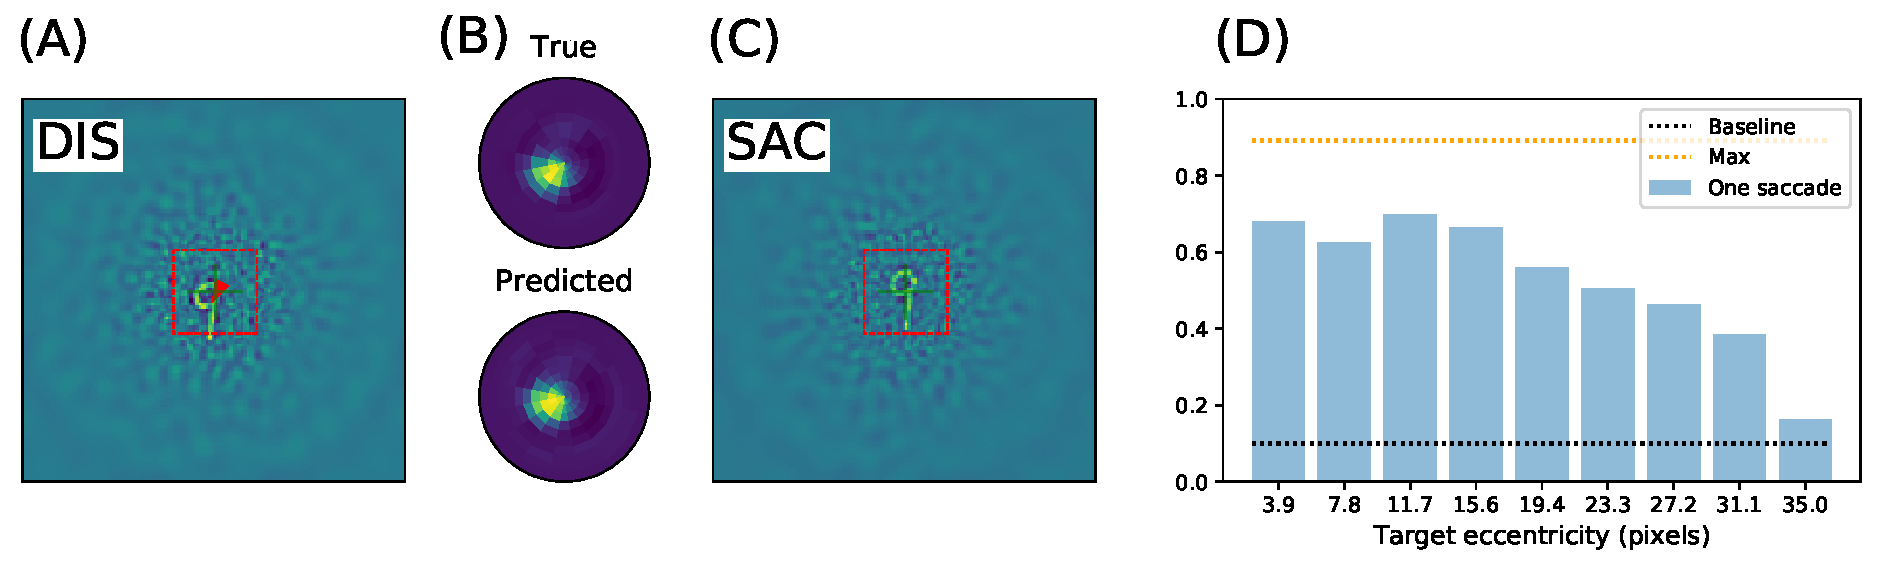
\includegraphics[width=\linewidth]{fig_result}}
\caption{
{\bf Simulated active vision agent}:
\A The visual display (\DIS , see also  Figure~\ref{fig:intro}-C)  is transformed into a retinotopic representation which is used as the input of a multi-layer neural network implementing the ``where'' pathway, that transforms the retinal image into an accuracy map. %
\B We show after training a typical network output  ('Predicted') as compared  with the ground truth ('True'). %
\C The network output allows to generate a saccade to the most likely target position in visual space and to recenter the retinotopic map (\SAC ), making possible to estimate a final classification rate. %
\D The active vision agent is tested at different eccentricities (in pixels). Orange bars: accuracy of a central classifier ('No saccade') with respect to the target's eccentricity, averaged over 1,000 trials per eccentricity scale. Blue bars: Final classification rate after one saccade predicted by the ``Where'' pathway.
\label{fig:results}}%
\end{figure}%
%%------------------------------%
% energy consumption

% inhibition of return
As our saccade selection algorithm may implement the essential operations done in the ``Where'' pathway, the central classifier may also reflect the response of the ``What'' pathway,
%A particular property of our agent is that at the time when the initial input is presented, two independent inferences are implemented. First, a
%The classification performed by the ``What'' pathway
giving the potential category of the digit. %Second, an accuracy map is predicted by the 'Where' pathway.
It is therefore possible to compare the two accuracy estimates to chose the most appropriate action: it may be that the  accuracy is best in the ``What'' pathway and in that case no saccade is produced.
The decision frontier lies between the first and the second spatial scale, allowing to pursue micro-saccades in the close vicinity of the target (2-3 pixels), in order to achieve a perfect centering.
In the other decision case, the ''What'' accuracy can still be considered to update the ``Where'' accuracy.
%Indeed, one knows in particular the accuracy of the 'what' pathway when imposing small shifts to the input.
This allows in particular to ``explain away" the current position of the fixation and the neighboring ones.
%(see line 'No saccade' in figure~\ref{fig:results}).
Such heuristic gives a principled formulation of the inhibition of return mechanism which is an important aspect for modeling saccades~\citep{Itti01}. In particular, we predict that such a mechanism is dependent on the class of inputs, and would be different for searching for faces as compared to digits.

\subsection{Quantitative role of parameters}
%=================================================================
%------------------------------%
%: see Figure~\ref{fig:params}
\begin{figure}[t!]%%[p!]
%\flushleft{\bf (A) \hspace{4.2cm} (B) \hspace{2cm} (C) \hspace{4cm} (D)\hspace{6cm}}
\centering{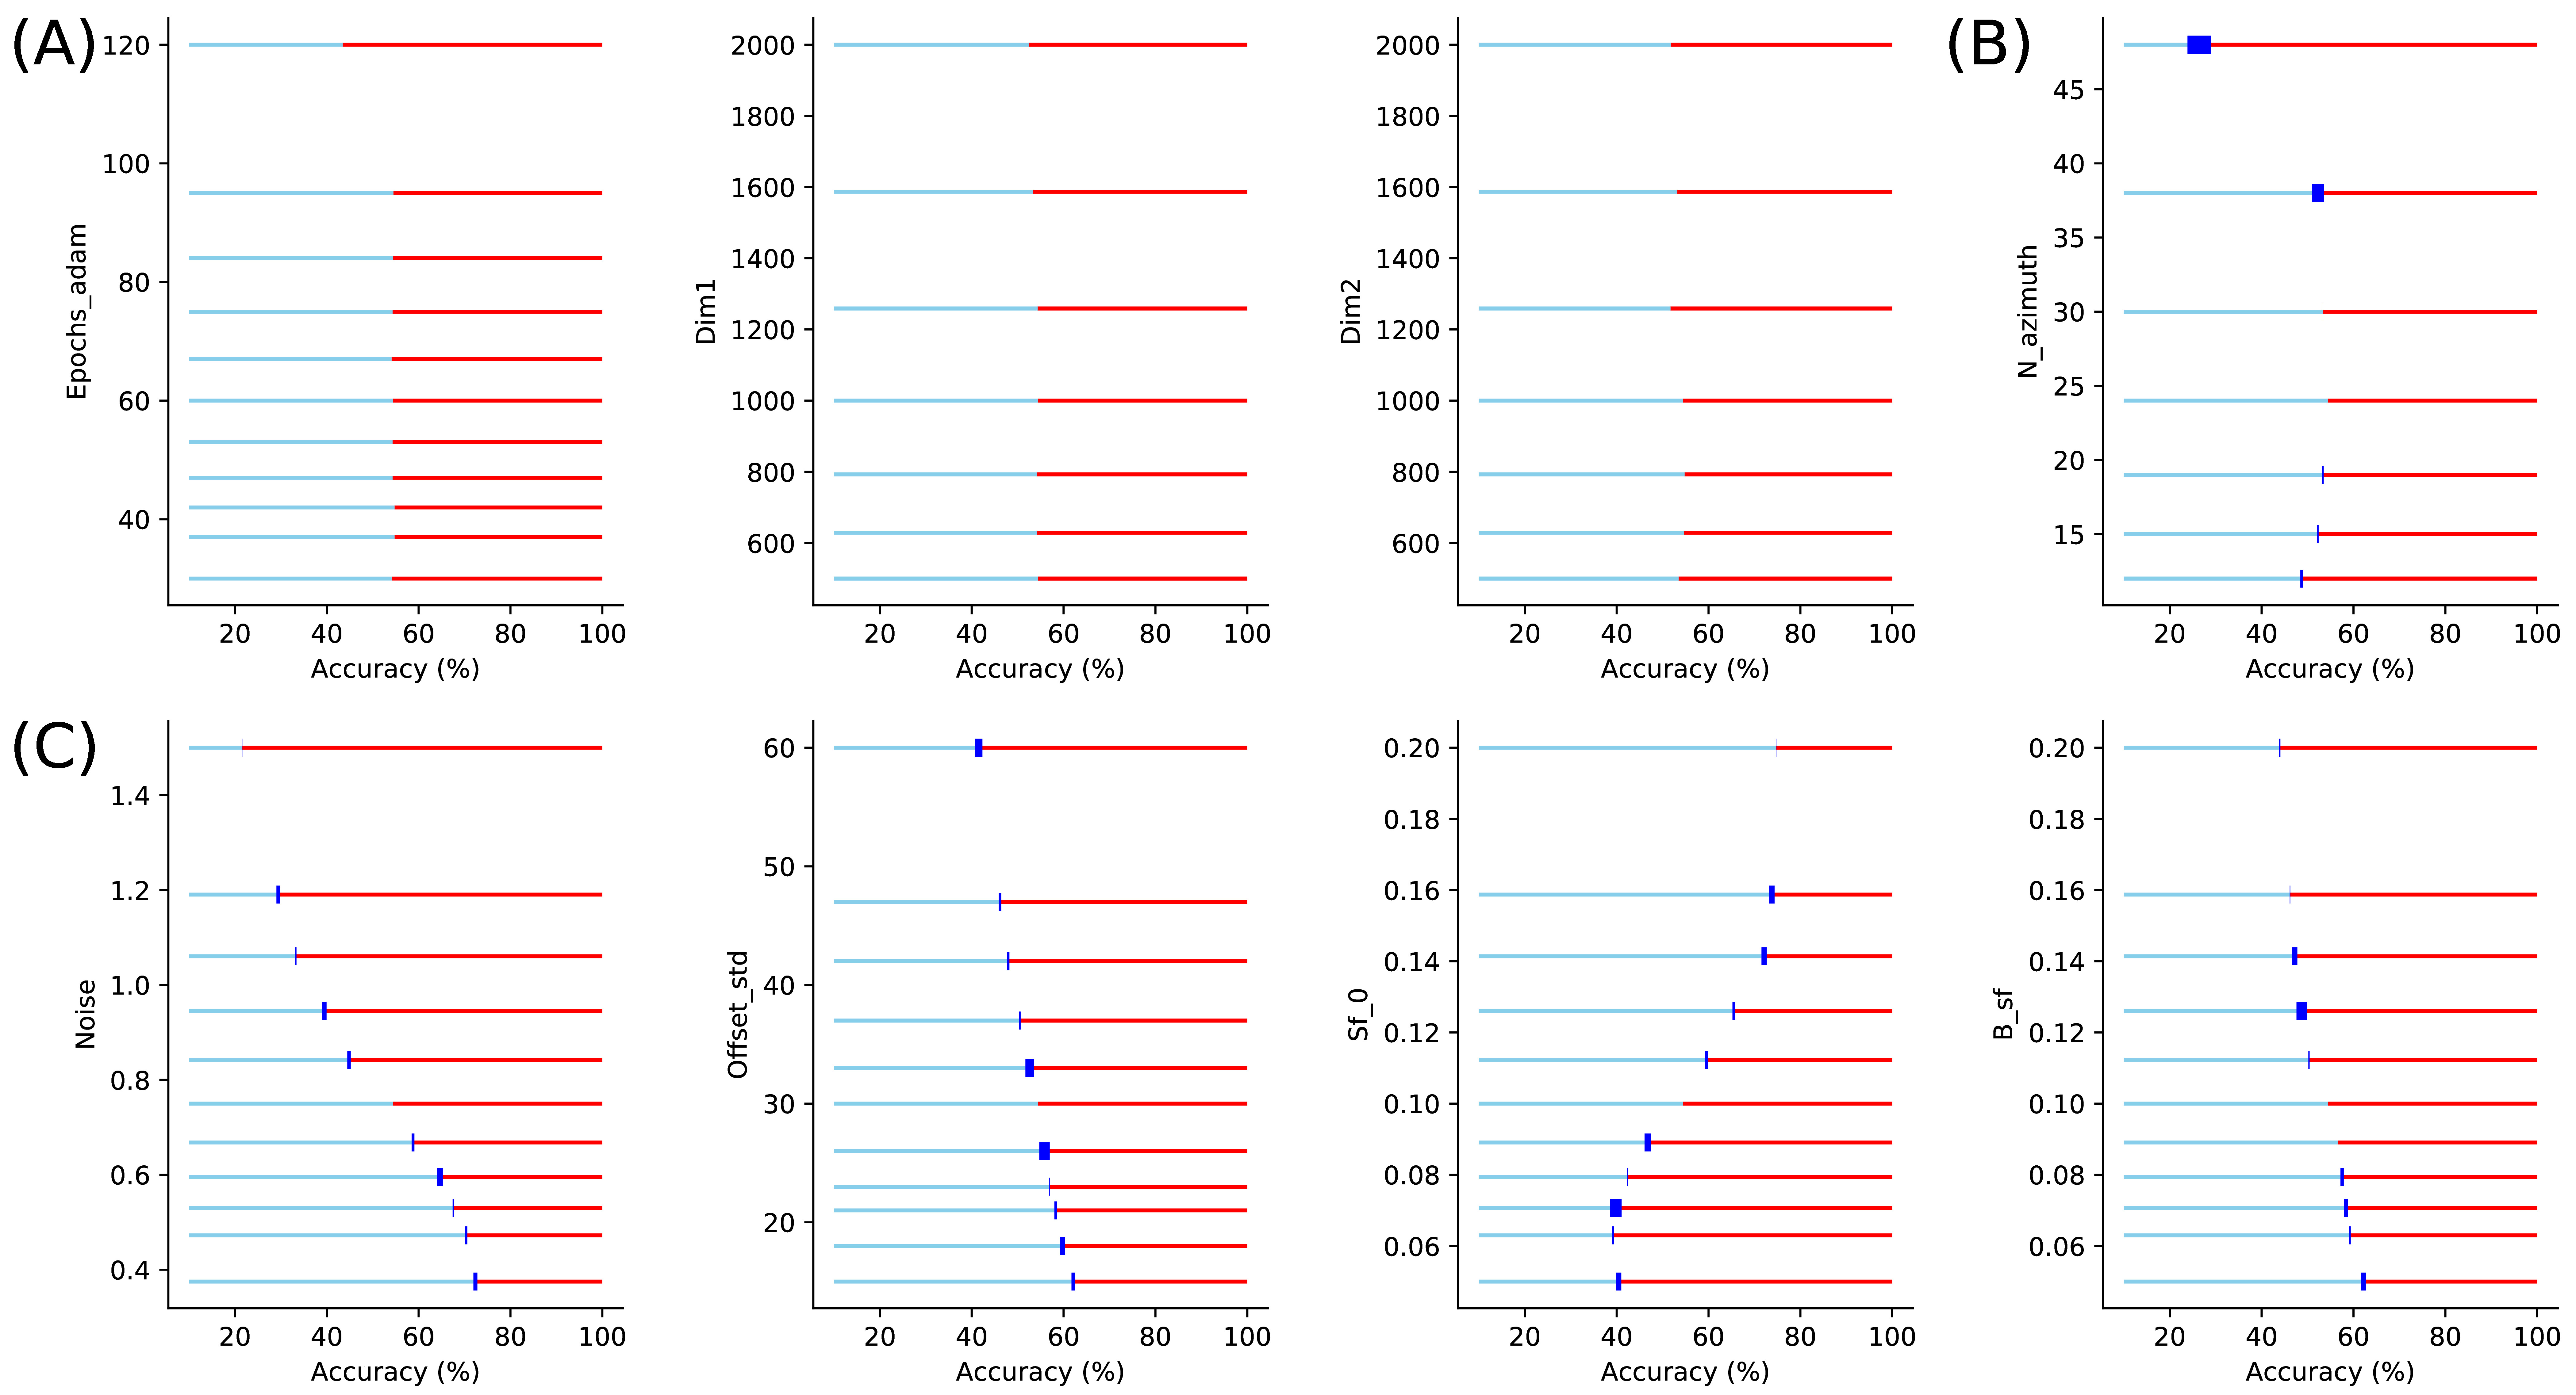
\includegraphics[width=\linewidth]{fig_params}}
\caption{
{\bf Quantitative role of parameters}: We show here variations of the average accuracy as a function of some free parameters of the model.  All parameters of the presented model were tested, from the architecture of image generation, to the parameters of the neural network implementing the ``Where'' pathway (including meta-parameters of the learning paradigm). We show here the results which show the most significative impact on average accuracy. %
\A First, we scanned parameters of the Deep Learning neural network. It shows that accuracy quickly converged after a characteristic time of approximately $25$ \texttt{epochs}. We then tested different values for the dimension of respectively the fist (\texttt{dim1}) and second (\texttt{dim2}) hidden layers, showing marginal changes in accuracy. %
\B The accuracy also changes with the architecture of the foveated input as shown here by changing the number \texttt{N\_azimuth} of azimuth directions which are sampled in visual space. This shows a compromise between a rough azimuth representation and a large precision, which necessitates a longer training phase., such that the optimal number is around $20$ azimuth directions. %
\C Finally, we tested some properties of the input, respectively from left to right: noise level (\texttt{noise}), mean spatial frequency of clutter \texttt{sf\_0} and bandwidth \texttt{B\_sf} of the clutter noise. This shows that average accuracy evolves with noise (see also Figure~\ref{fig:results} for an evolution as a function of eccentricity), but also to the characteristics of the noise clutter. In particular, there is a drop in accuracy whenever noise is of similar wavelength as digits, but which becomes less pronounced as the bandwidth increases. %
\label{fig:params}}%
\end{figure}%
%%------------------------------%
